\documentclass{ikpKoeln}
\usepackage{graphicx}
\usepackage{physics}
\usepackage{xcolor}
\usepackage{tikz}
\usepackage{siunitx}
\usepackage[font=normalsize,skip=0pt]{caption}
\usepackage{luacode}
\usetikzlibrary{math, shapes.geometric, arrows, positioning, decorations.markings}

\scTitle{An overview of data calibration algorithms of NeuLAND\\ in the R$^3$B setup}
\scAuthor{*}{Yanzhao}{Wang}{1}
\scAuthor{}{Paula}{Ulrich}{1}
\scAuthor{}{Igor}{Gasparic}{2}
\scAuthor{}{Andreas}{Zilges}{1}
\scAffiliation{1}{University of Cologne, Institute for Nuclear Physics, Germany}
\scAffiliation{2}{GSI Helmholtzzentrum für Schwerionenforschung, Germany}
\scEmail{ywang@ikp.uni-koeln.de}

\scTitleShort{Data calibration algorithms of NeuLAND}

\date{\scriptsize HK 44.4 \\DPG-Frühjahrstagung\\Cologne 2025 \\ \vspace{1em} Supported by BMBF (05P24PK1)}

\graphicspath{{../figures/}}

\DeclareSourcemap
{
    \maps[datatype=bibtex,overwrite=true]
    {
        \map{
        \step[fieldsource=journal,
           match={Nuclear Instruments and Methods in Physics Research, Section A: Accelerators, Spectrometers, Detectors, and Associated Equipment},
           replace={Nucl. Instrum. Methods Phys. Res., Sect. A}]
            }
    }
}

\addbibresource{reference.bib}

\AtBeginDocument{\RenewCommandCopy\qty\SI}

\begin{document}

{
\usebackgroundtemplate{%
	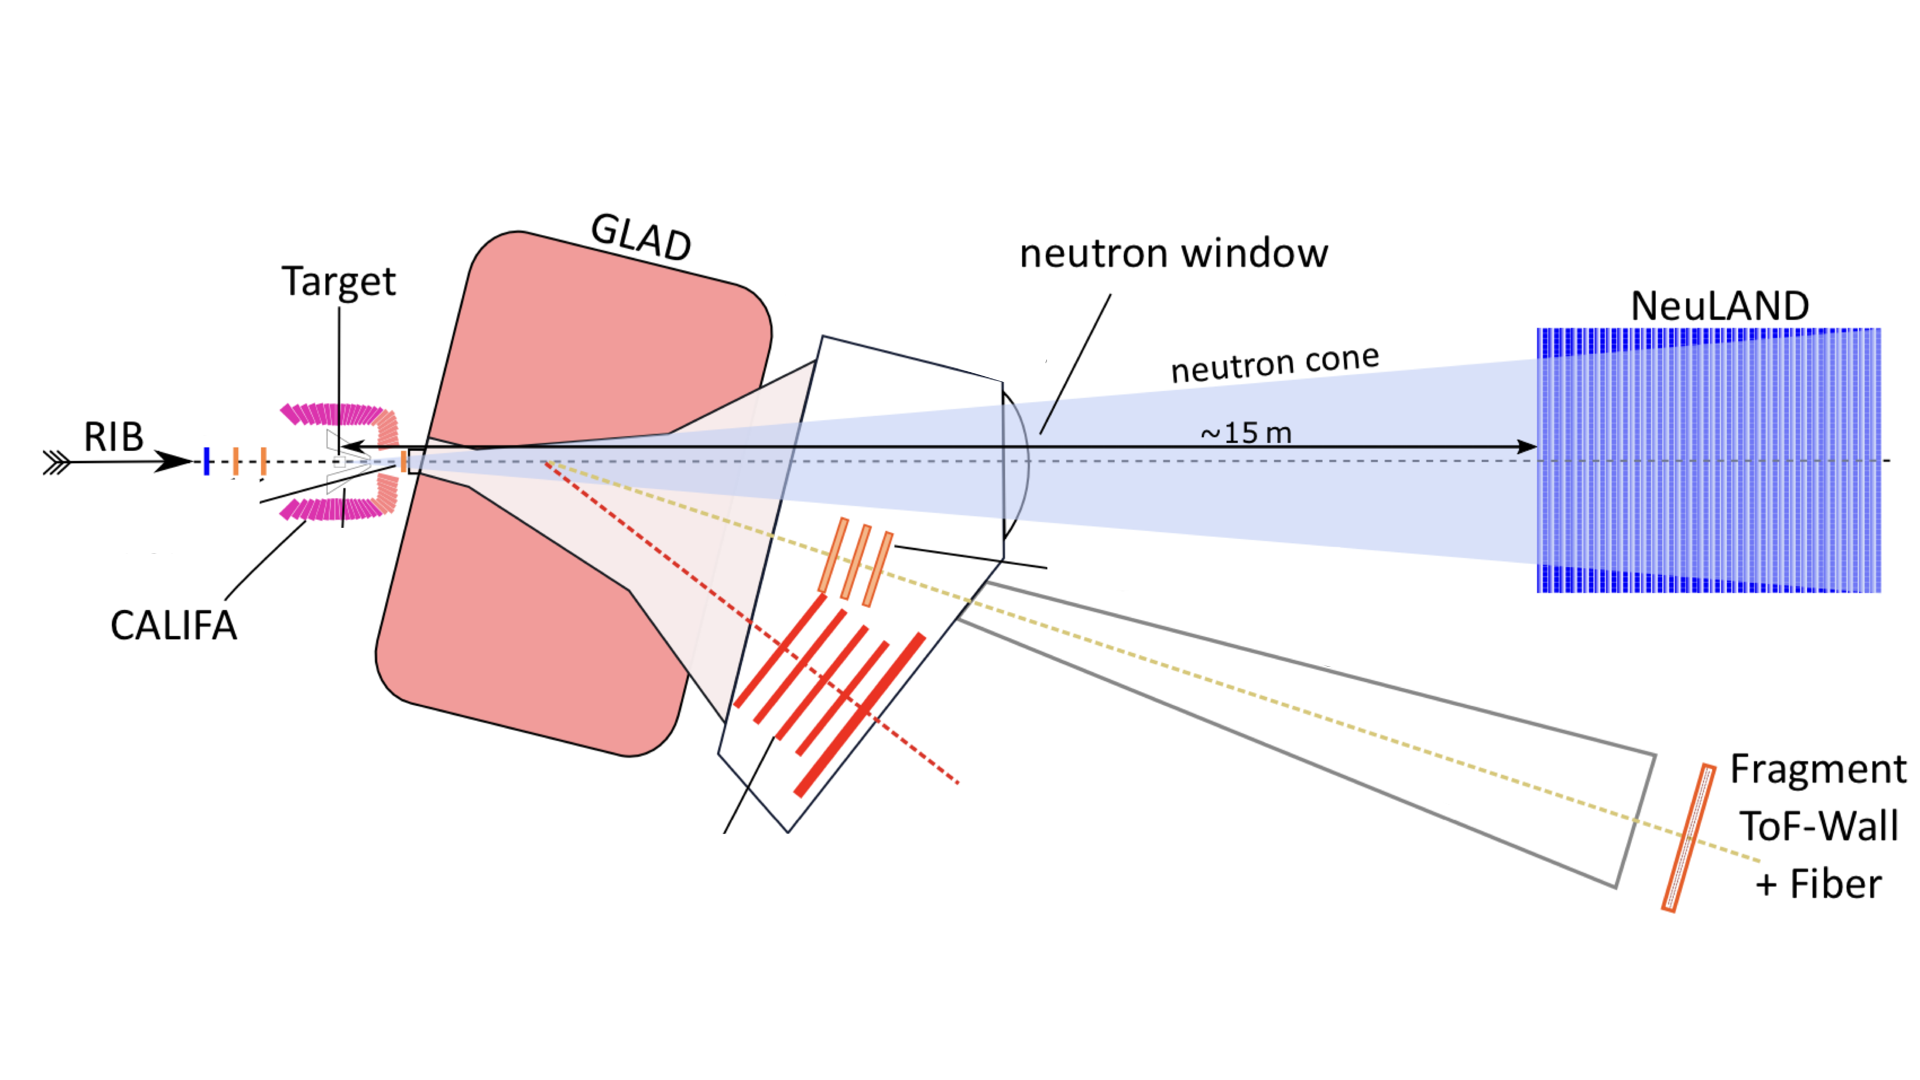
\includegraphics[width=\paperwidth, height=\paperheight]{r3b/r3bsetup_empty.png}}
\begin{frame}{NeuLAND setup in $\text{R}^3\text{B}$\footfullcite{BORETZKY}}

	\begin{columns}[c]
		\begin{column}{0.4\textwidth}
			\pause
			\begin{figure}
				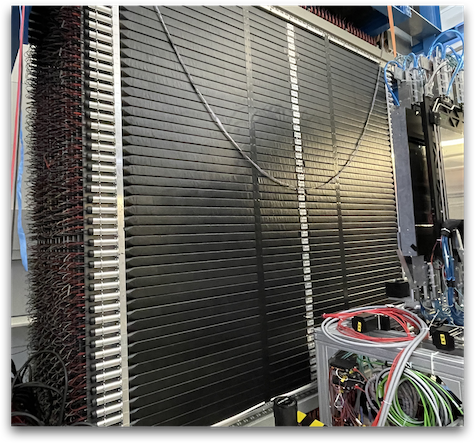
\includegraphics[width = \textwidth]{neuland/neulandReal}
			\end{figure}
		\end{column}
		\hspace*{0.5cm}
		\begin{column}{0.3\textwidth}
			\begin{exampleblock}{}
				Geometry:\\
				\begin{itemize}
					\item $26$ planes
					\item $\qtyproduct[product-units=power]{250 x 250}{\centi\meter}$
					\item $50$ scintillators each plane
					\item $2600$ PMTs in total
				\end{itemize}
				\pause
				Measurements:\\
				\begin{itemize}
					\item interaction position
					\item interaction time
					\item energy deposition
				\end{itemize}
			\end{exampleblock}
		\end{column}
		\begin{column}{0.3\textwidth}
		\end{column}
	\end{columns}
	% \let\thefootnote\relax\footnotetext{\fullcite{BORETZKY}}
\end{frame}
}

\begin{frame}[t]{Processes of digitization}
	\begin{columns}
		\begin{column}{0.4\textwidth}
			\hspace*{-1.5em}\textbf{\textit{Physical interactions}}:
			\begin{figure}[t]
				\hspace*{-5em}
				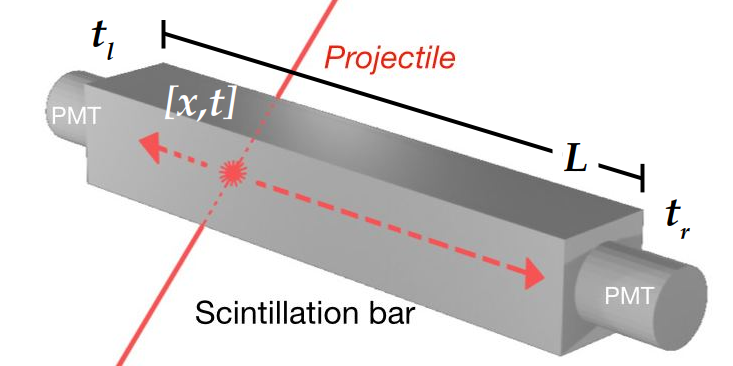
\includegraphics[width = 0.8\textwidth]{R3BCon2024GSI/Bar.png}
			\end{figure}
			\vspace{1em}
			\hspace*{-1.5em}\textbf{\textit{Digitization of PMT signals}}:
			\begin{figure}
				\hspace*{-5em}
				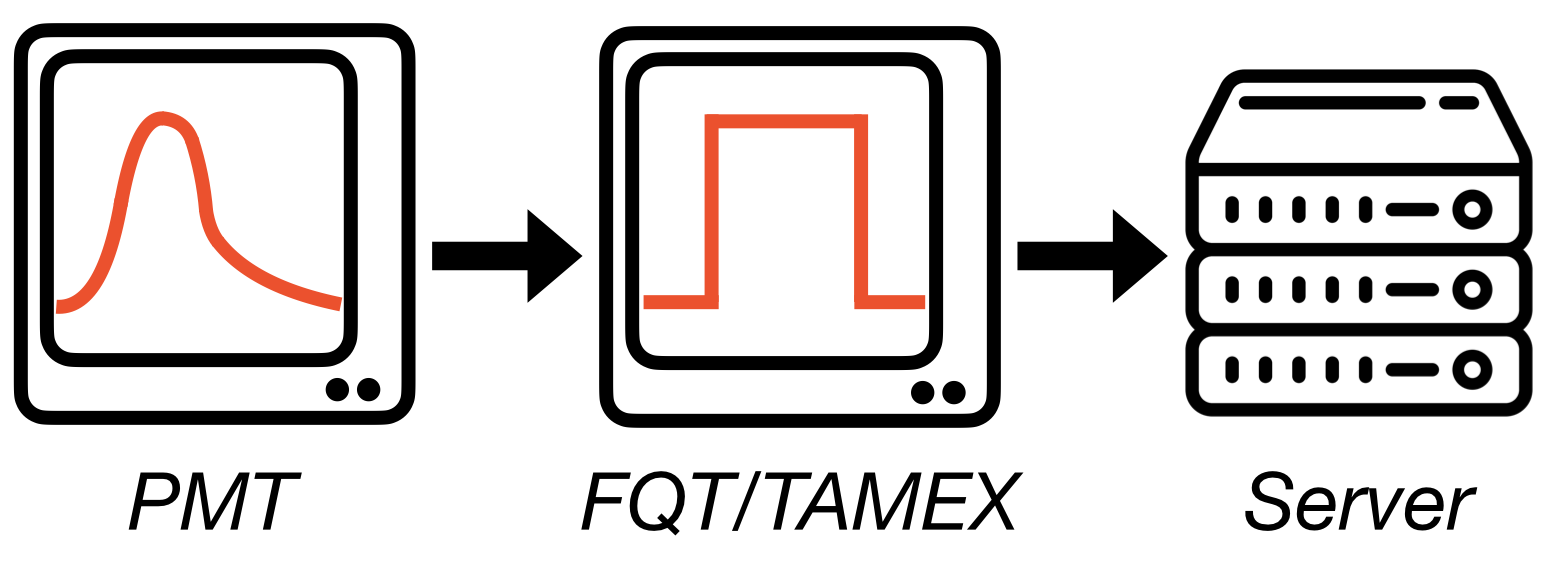
\includegraphics[width = 0.8\textwidth]{neuland/PMT2TAMEX}
			\end{figure}
		\end{column}
		\begin{column}{0.5\textwidth}
			\def\largeWidth{7cm}
			\def\smallWidth{2.5cm}
			\hspace*{-2em}
			\begin{tikzpicture} [node distance=2cm]
				\tikzstyle{lineWidth} = [line width = 0.5mm]
				\tikzstyle{dataformat} = [rectangle, rounded corners, minimum width=\largeWidth, minimum height=0.7cm, text centered, draw = black, lineWidth];
				\tikzstyle{process} = [ellipse, minimum width=3cm, minimum height=0.7cm, text centered, draw = red, lineWidth];
				\tikzstyle{arrow} = [thick, ->, >=stealth]

				\node (physical)[dataformat]{Physical data (energy, time and position)};
				\node (pmt)[process, below left =1cm and -\smallWidth of physical]{PMT, FQT};
				\node (signal)[dataformat, below = 2.5cm of physical,]{Logic signals (leading and trailing edges)};
				\node (tamex)[process, below left =1cm and -\smallWidth of signal]{TAMEX};
				\node (second-cal)[process, inner sep = 0mm, below right =1cm and -\smallWidth of physical, xshift = -1.5em]{2nd calibrations};
				\node (tdc)[process, inner sep = 0mm, below right =1cm and -\smallWidth of signal, xshift=-1.5em]{1st calibration};
				\node (TDCData)[dataformat, below = 2.5cm of signal]{TDC (channels, module IDs, etc.)};

				\draw [arrow] (pmt.north |- physical.south) -- (pmt.north);
				\draw [arrow] (second-cal.north) -- (second-cal.north |- physical.south);
				\draw [arrow] (pmt.south) -- (pmt.south |- signal.north);
				\draw [arrow] (second-cal.south |- signal.north) -- (second-cal.south);
				\draw [arrow] (tamex.north |- signal.south) -- (tamex.north);
				\draw [arrow] (second-cal.south |- tdc.north) -- (second-cal.south |- signal.south);
				\draw [arrow] (tamex.south) -- (tamex.south |- TDCData.north);
				\draw [arrow] (second-cal.south |- TDCData.north) -- (second-cal.south |- tdc.south);

				\begin{scope}[decoration={
								markings,
								mark=at position 0.5 with {\arrow[scale=2, >=stealth]{>}}}
					]
					\draw [dashed, -,  postaction={decorate}](physical.west) -- ([xshift=-0.5em]physical.west) -- node[above, rotate = 90]{\textbf{\textit{Data digitization}}}([xshift=-0.5em]TDCData.west) -- (TDCData.west);
					\draw [dashed, -,  postaction={decorate}](TDCData.east) -- ([xshift=0.6em]TDCData.east) -- node[above, rotate = -90]{\textbf{\textit{Data calibration}}}([xshift=0.6em]physical.east) -- (physical.east);
				\end{scope}
			\end{tikzpicture}
		\end{column}
	\end{columns}
\end{frame}

\begin{frame}[t]{Time measurement and TDC calibration}
	\vspace{-0.5em}
	\begin{columns}[c]
		\begin{column}{0.45 \textwidth}
			\def\upperHeight{1.5cm}
			\def\lowerHeight{1cm}
			\def\totalWidth{5cm}
			\def\clockWidth{10mm}
			\def\clockHight{9mm}
			\def\signalPos{33mm}
			\def\CTHeight{-5mm}

			\vspace{-2em}
			\begin{figure}
				\captionsetup{singlelinecheck=off,font=normalsize}
				\caption*{\textbf{\textit{Time measurement with clocks:}}}
				\vspace{-0.5em}
				\begin{tikzpicture}
					\draw [<-, >=stealth](0, \upperHeight) node[above, rotate=90]{\textit{\scriptsize CLK}}-- (0, -\lowerHeight);
					\draw [->, >=stealth](0, 0) -- node[very near end, below]{\scriptsize time}(\totalWidth, 0);

					\draw[thick] (0,0)
					\foreach \x in {1,...,2}{
							-- ++(0,\clockHight) -- ++(\clockWidth, 0) -- ++(0,-\clockHight) -- ++(\clockWidth,0)
						} -- ++(0,\clockHight) -- ++(\clockWidth, 0);
					\draw[thick, dashed] (\signalPos, \upperHeight) -- node[left, very near start, yshift = 1em]{trigger}(\signalPos, -\lowerHeight);
					\draw[thick, ->, >=stealth, red] (0, \CTHeight) -- node[below]{Coarse time} (40mm, \CTHeight);
					\draw[thick, <->, >=stealth, red] (\signalPos, -\CTHeight) -- node[above, yshift = 1.3em, xshift = 1.2em, name=fineTime]{Fine time} (40mm, -\CTHeight);
					\draw[red]({0.5*\signalPos + 20mm}, -\CTHeight) -- ([xshift=-1em]fineTime.south);
					\draw[thick, red] (40mm, {\CTHeight+1mm}) -- (40mm, {\CTHeight-1mm});
				\end{tikzpicture}
			\end{figure}

			\textbf{\textit{Real time calculation:}}

			\vspace{-0.5em}
			$$T_\text{real} = T_\text{coarse} - T_\text{fine}$$
			\vspace{-1em}
			\small
			{
				\begin{itemize}
					\item $T_\text{real}$: Time value relative to START detector
					\item $T_\text{coarse}$: Clock cycles with a frequency of $\qty{200}{\MHz}$ ($\text{period} = \qty{5}{\nano\second}$)
					\item $T_\text{fine}$: Fine channel numbers (TDL)
				\end{itemize}
			}
		\end{column}
		\begin{column}{0.5 \textwidth}
			\begin{figure}
				\vspace{-0.8em}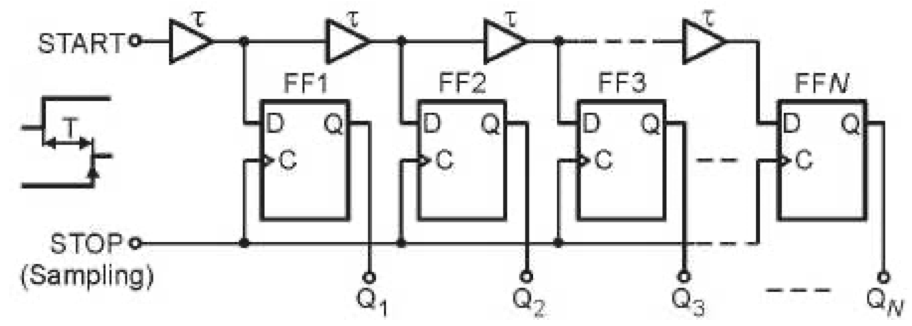
\includegraphics[width = \textwidth]{r3b/TDCFineTime}
				\caption*{Tapped Delay Line (TDL)\footfullcite{TDCFINETIME}}
				\onslide<2>{
					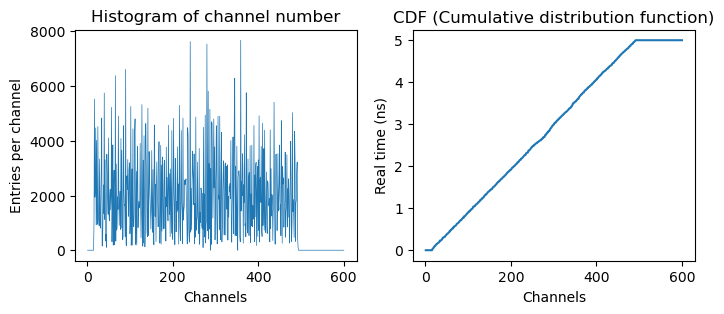
\includegraphics[width = \textwidth]{neuland/FineTimeCal}
					\caption*{TDC Calibration (Time resolution $\sim \qty{10}{\pico\second}$)}
				}
			\end{figure}
			\vspace{-2.3em}
		\end{column}
	\end{columns}
\end{frame}

\begin{frame}[t]{Position calibration from cosmic muons}
	\vspace {-2.5em}
	\begin{columns}[t]
		\begin{column}{0.45 \textwidth}
			\begin{block}{Calibration relations}
				\setlength{\abovedisplayskip}{0pt}
				\setlength{\belowdisplayskip}{0pt}
				\setlength{\abovedisplayshortskip}{0pt}
				\setlength{\belowdisplayshortskip}{0pt}
				\begin{flalign}
					\intertext{Interaction position:}
					x & = \frac{\alert{C_e}}{2}\left( t_r - t_l  + \alert{t_\text{offset}} \right)    \\
					\intertext{Interaction time:}
					t & = \frac{t_r + t_l}{2} - \frac{L}{2 \cdot \alert{C_e}} + \alert{t_\text{sync}}
				\end{flalign}
			\end{block}
			\begin{exampleblock}{Position calibration steps}
				\begin{enumerate}
					\setlength\itemsep{0em}
					\setbeamercovered{transparent}
					\item<1-> Collect time difference values of adjacent PMT signals from cosmic muons
					\item<2-> Normalize the distribution and convert to the CDF for each bar
					\item<3-> Linear fitting of the CDF within its quantiles of 0.05 to 0.95
				\end{enumerate}
			\end{exampleblock}
		\end{column}
		\begin{column}{0.45 \textwidth}
			\begin{figure}
				\captionsetup{singlelinecheck=off}
				\caption*{\textit{\textbf{Parameter fitting:}}}
				\vspace*{-0.5em}
				\includegraphics<1>[width = 0.9\textwidth]{DPG2025/TimeDifference_0.png}%
				\includegraphics<2>[width = 0.9\textwidth]{DPG2025/TimeDifference_1.png}%
				\includegraphics<3>[width = 0.9\textwidth]{DPG2025/TimeDifference_2.png}%
			\end{figure}
			\onslide<3->
			{
				\setlength{\abovedisplayskip}{0pt}
				\setlength{\belowdisplayskip}{0pt}
				\setlength{\abovedisplayshortskip}{0pt}
				\setlength{\belowdisplayshortskip}{0pt}
				\vspace{-1em}
				\begin{flalign*}
					\intertext{Fitting function:}
					y               & = a \cdot x + 0.5 - a \cdot b       \\
					\intertext{Calculation of parameters:}
					C_e             & = 2 \cdot a \cdot \text{bar length} \\
					t_\text{offset} & = b
				\end{flalign*}
			}
		\end{column}
	\end{columns}
\end{frame}

\begin{frame}[t]{Current energy calibration method (WIP)}
	\setcounter{equation}{0}
	\vspace*{-0.5em}
	\begin{columns}[c]
		\begin{column}{0.45 \textwidth}
			\vspace{-1.5em}
			\begin{alertblock}{Energy calibration relations}
				\setlength{\abovedisplayskip}{0pt}
				\setlength{\belowdisplayskip}{0pt}
				\setlength{\abovedisplayshortskip}{0pt}
				\setlength{\belowdisplayshortskip}{0pt}
				\begin{flalign}
					\intertext{PMT signal amplitude:}
					I_\text{PMT} & = E_\text{dep} \cdot \exp(-\alert{\alpha} \cdot l)                                           \\
					\intertext{Applying PMT saturation effect:}
					I_\text{sat} & = \left. I_\text{PMT} \middle/ \left( 1 + \alert{\lambda} \cdot I_\text{PMT} \right) \right. \\
					\intertext{Logic signal width:}
					W            & = \alert{\mathcal{G}} \cdot I_\text{sat} + \alert{W_0}
				\end{flalign}
			\end{alertblock}
			\vspace{-0.5em}
			\begin{exampleblock}{Assumptions}
				\begin{itemize}
					\setlength\itemsep{0em}
					\item PMT saturation factor is proportional to the gain factor: \vspace{-1em}$$\alert{\lambda} = 0.00175 \times \alert{\mathcal{G}}$$
					\item \vspace{-1em}Cosmic muon's stopping power is \qty{1.73}{\mega\electronvolt\per\centi\metre}
					\item Adjacent PMTs have the same gain factor
				\end{itemize}
			\end{exampleblock}
		\end{column}
		\begin{column}{0.45 \textwidth}
			\textit{\textbf{Calculation of parameters:}}
			{\small
				\begin{itemize}
					\setlength\itemsep{0em}
					\item Signal width baseline $\alert{W_0}$ is determined by the minimum cut on signal widths (i.e. trailing time $-$ leading time).
					\item Calculation of attenuation factor:
					      \vspace{-0.5em}
					      $$ \left. \alert{\alpha} = \ln((W_r - W_0) \middle/ (W_l - W_0)) \middle/ (2 \cdot x) \right.$$
					\item \vspace{-1em}Calculation of gain factor:
					      \vspace{-0.5em}
					      $$\alert{\mathcal{G}} = \frac{W - \alert{W_0}}{I_\text{PMT} \left(1 - 0.00175(W - \alert{W_0})\right)}$$
				\end{itemize}
			}
			\begin{figure}
				\captionsetup{singlelinecheck=off}
				\vspace{-2em}
				\caption*{\textit{\textbf{PMT gains from all events:}}}
				\vspace{-1em}
				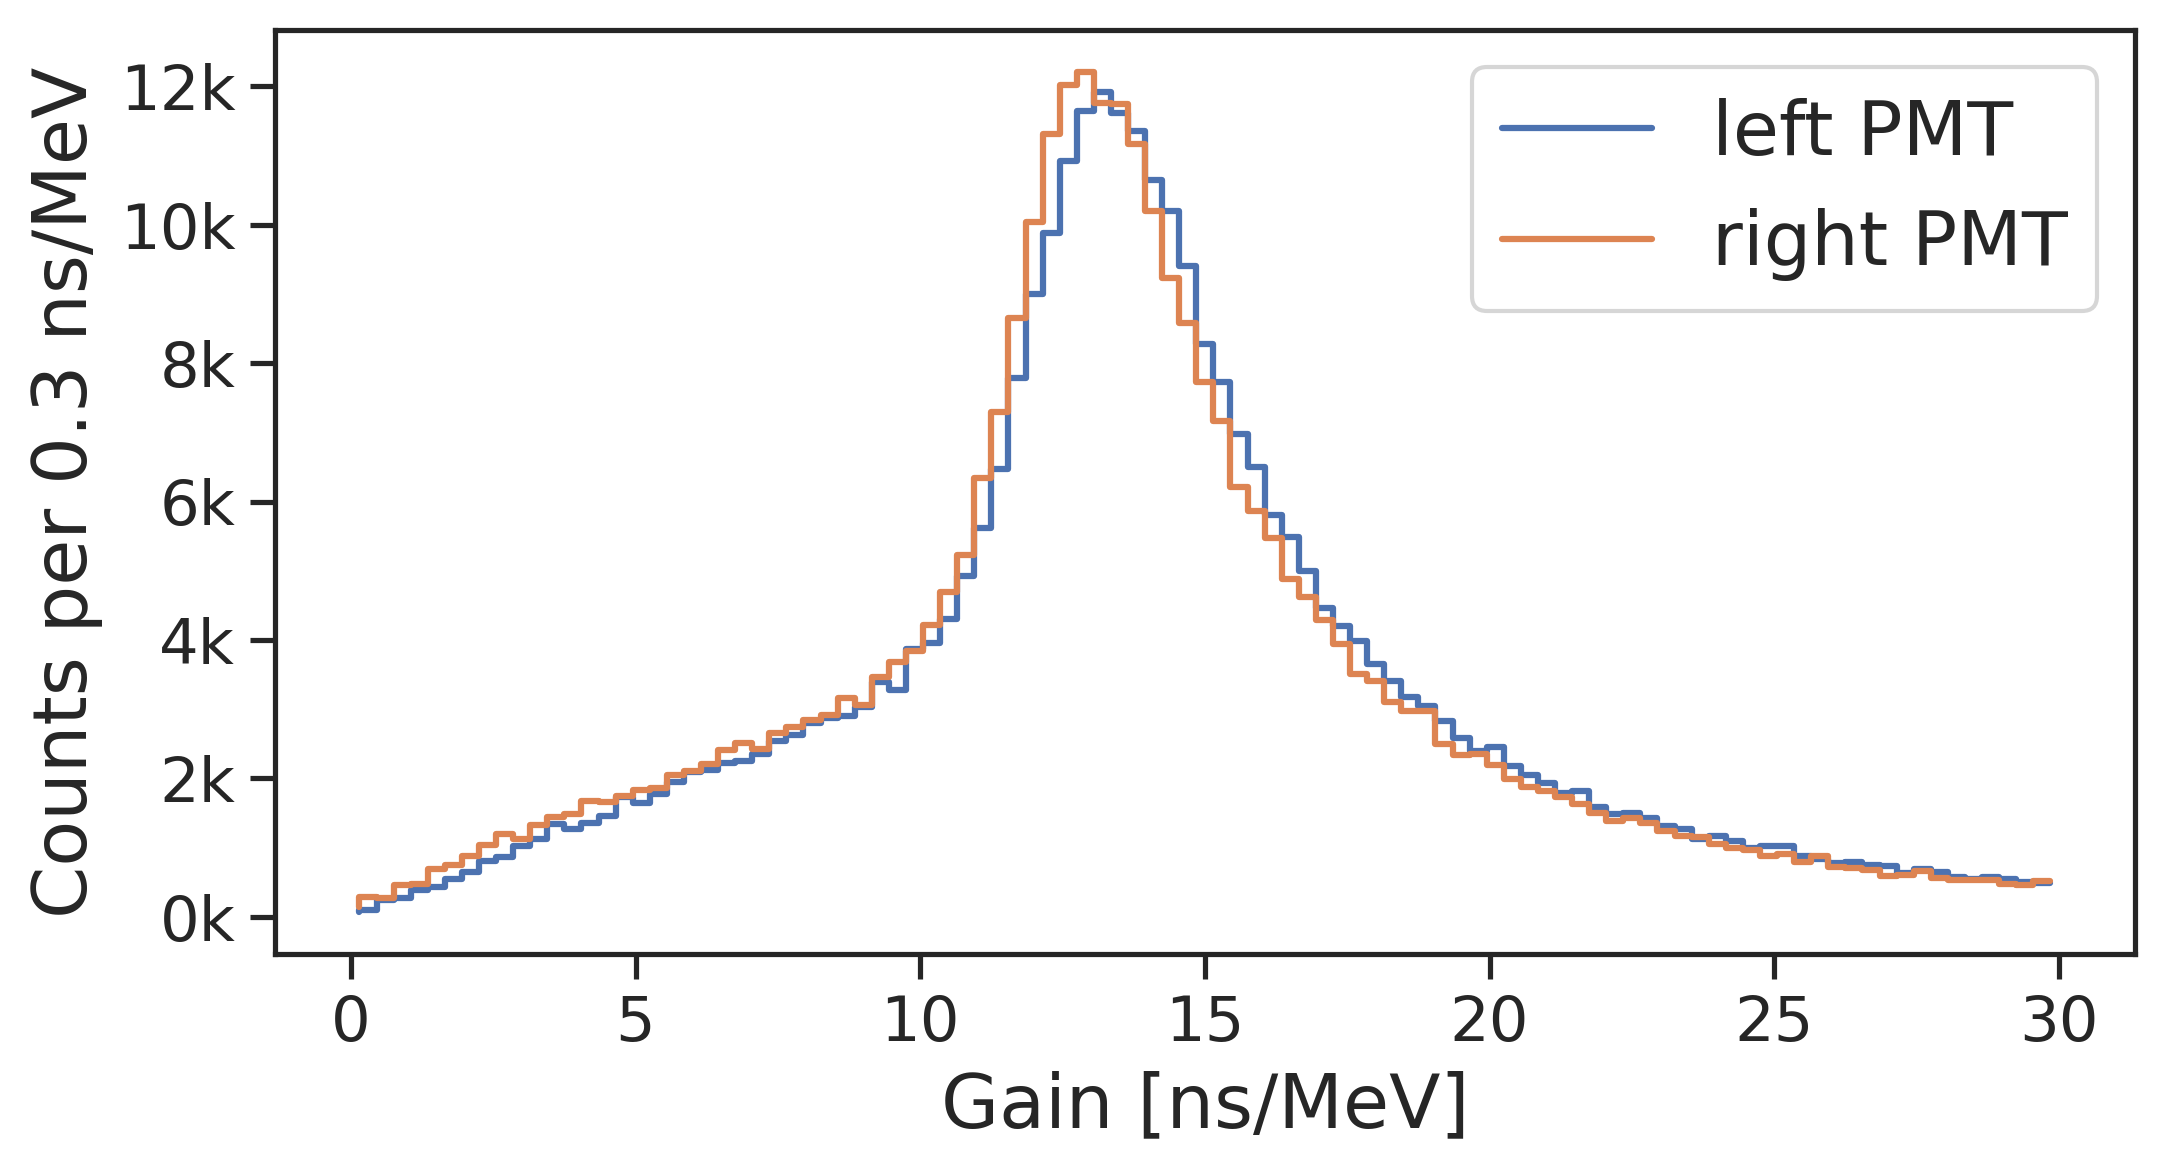
\includegraphics[width = 0.9\textwidth]{DPG2025/EnergyGain.png}
			\end{figure}
		\end{column}
	\end{columns}
\end{frame}

\begin{frame}[t]{Parameter fine tuning with Millepede-II}
	\vspace{-2em}
	\begin{columns}[t]
		\begin{column}{0.45 \textwidth}
			\begin{exampleblock} {Characteristics}
				\begin{itemize}
					\item Simultaneous fitting of all parameters
					\item Separation to global and local parameters
					\item Computation complexity independent of local parameter size
					\item \alert{\textbf{No particle track reconstruction}}
					\item Calibration relation \textbf{must be linear}
				\end{itemize}
			\end{exampleblock}

			\begin{figure}
				\vspace{-0.5em}
				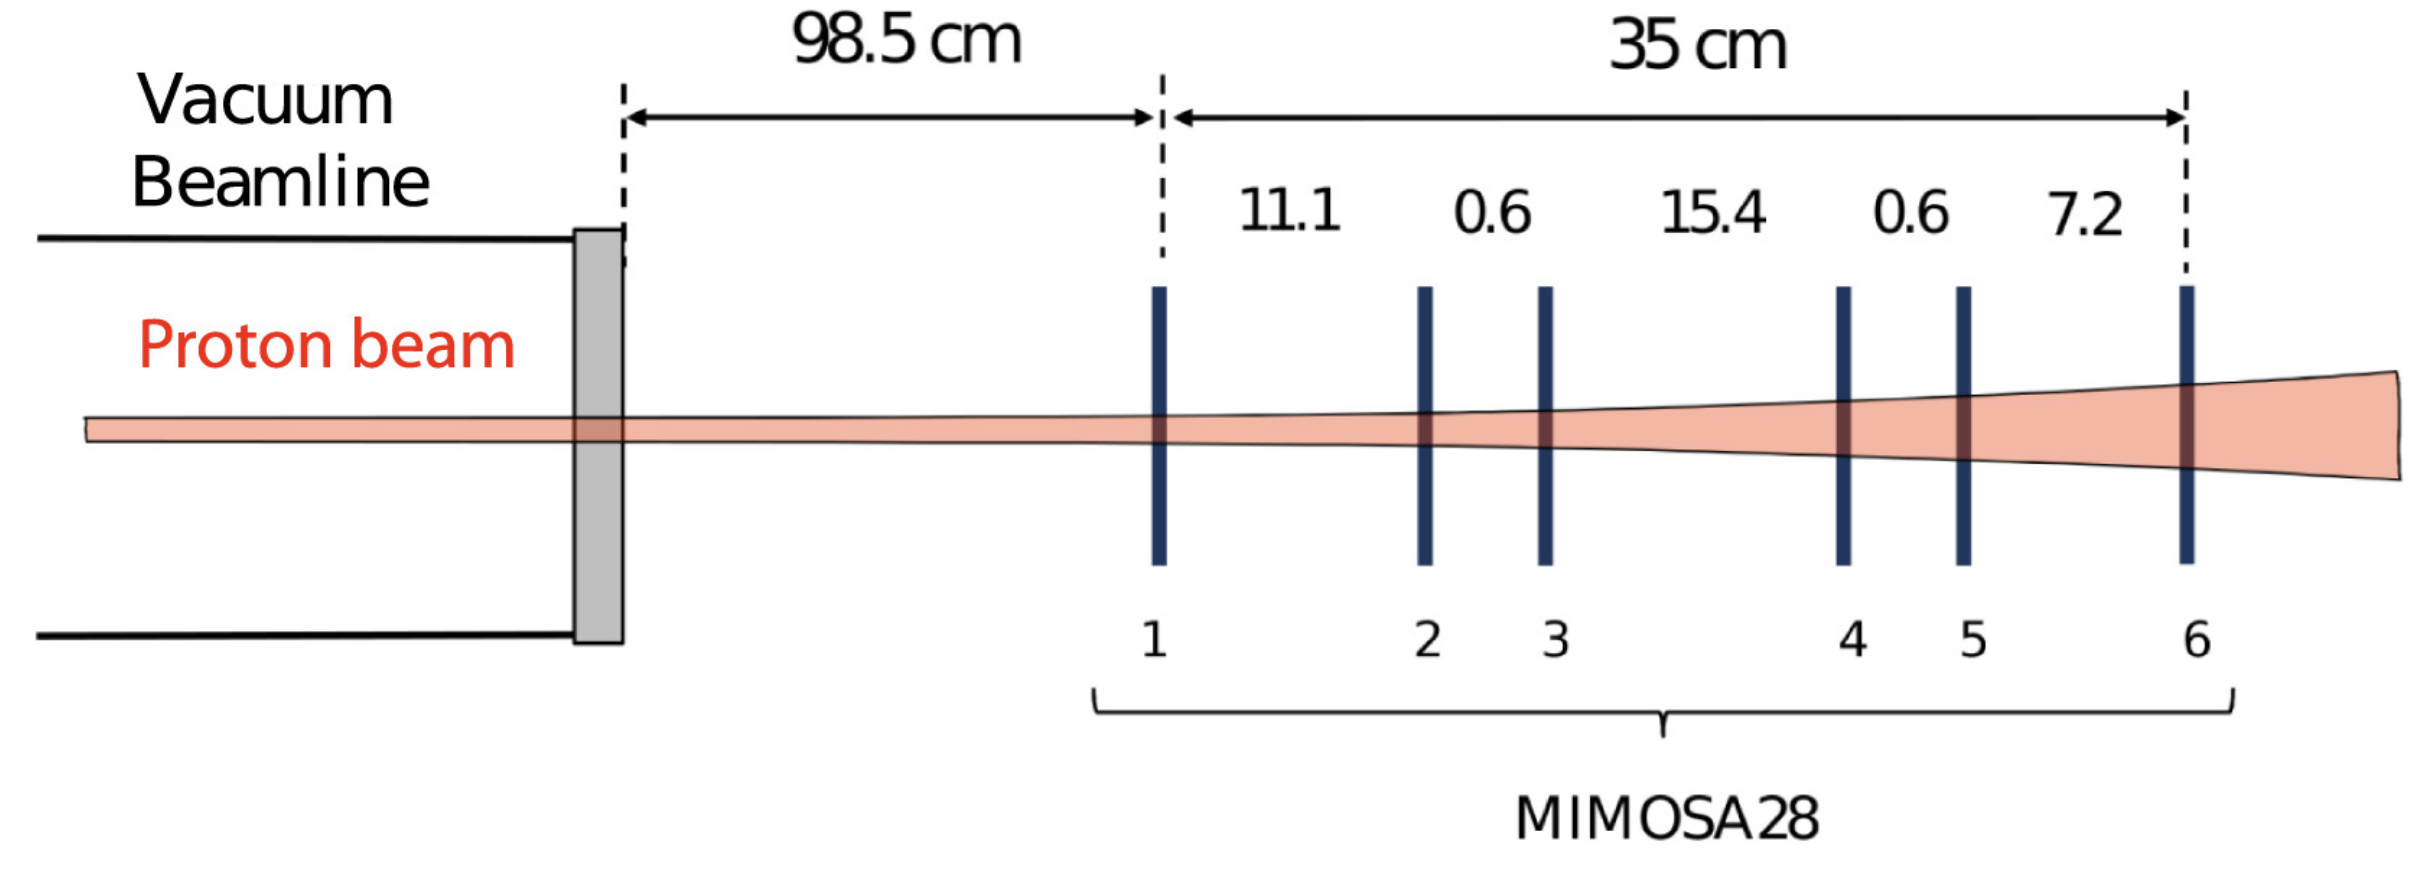
\includegraphics[width =\textwidth]{DPG2025/SilliconPixel.png}
				\caption*{Alignment of silicon pixel detectors \footfullcite{REIDEL2019142}}
			\end{figure}
			\vspace{-2.2em}
		\end{column}
		\begin{column}{0.45 \textwidth}
			\pause
			\begin{figure}
				\captionsetup{singlelinecheck=off}
				\caption*{Parameter fine tuning on $C_e$ in NeuLAND:}
				\vspace{-0.5em}
				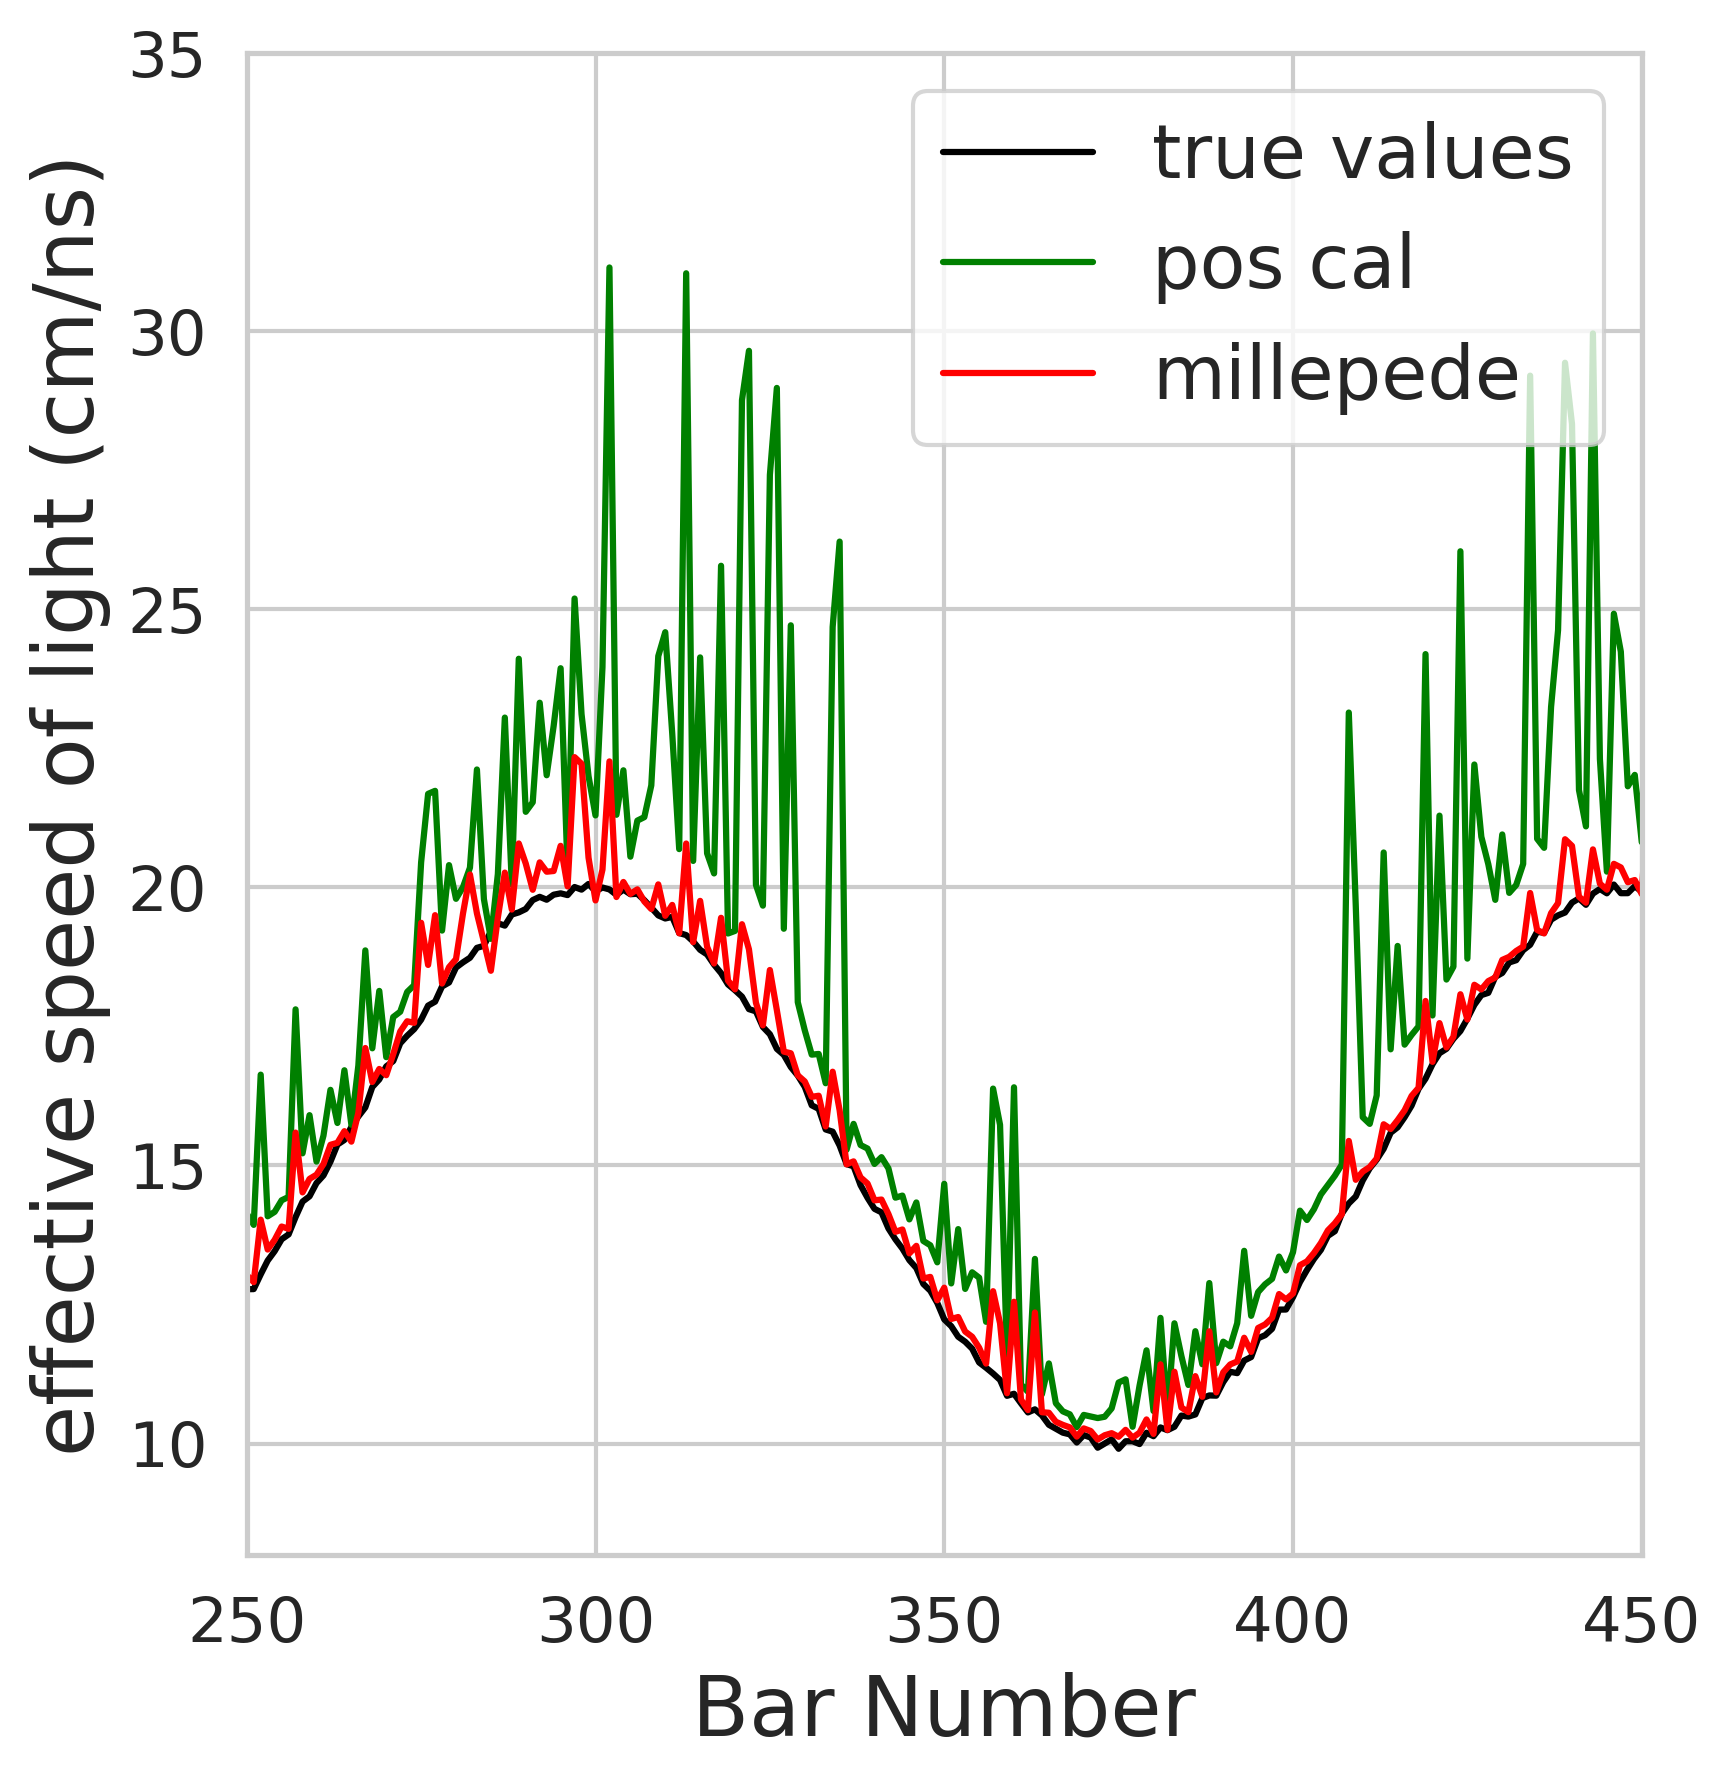
\includegraphics[width = \textwidth]{DPG2025/sim_comp_c.png}
			\end{figure}
		\end{column}
	\end{columns}
\end{frame}

\begin{frame}[t]{Summary and outlook}
	\vspace{-1em}
	\begin{columns}[c]
		\begin{column}{0.45 \textwidth}
			\begin{block} {Summary}
				\begin{itemize}
					\setlength\itemsep{0.5em}
					\item Principle of digitization processes
					\item Calibration with TDC for time values
					\item Calibration with time values for physical values
					\item Fine tuning with the Millepede-II algorithm
				\end{itemize}
			\end{block}
			\begin{exampleblock} {Outlook}
				\begin{itemize}
					\setlength\itemsep{0.5em}
					\item Improve energy calibration
					\item Apply Millepede-II algorithm on energy-related parameters
					\item Verify energy parameters via simulation
				\end{itemize}
			\end{exampleblock}
		\end{column}
		\begin{column}{0.45 \textwidth}
			\begin{figure}
				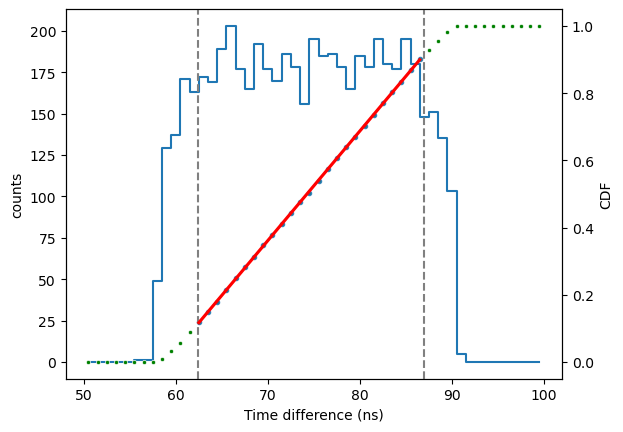
\includegraphics[width = 0.8\textwidth]{neuland/position_cal/TimeDifference4.png}
				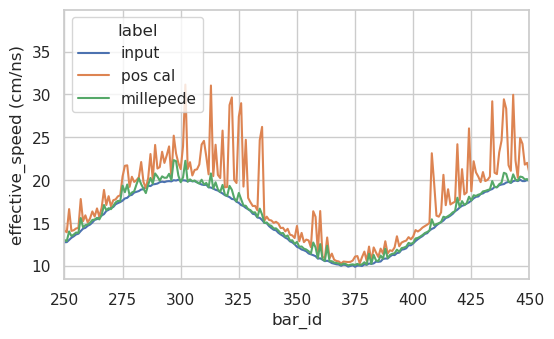
\includegraphics[width = 0.9\textwidth]{neuland/millepede/sim_eff_c.png}
			\end{figure}
		\end{column}
	\end{columns}
\end{frame}

% \begin{frame}[t]{Current position calibration}
% 	\vspace*{-2em}
% 	\begin{columns}[t]
% 		\begin{column}{0.45 \textwidth}
% 			\begin{figure}[t]
% 				\includegraphics<1>[width = \textwidth]{R3BCon2024GSI/side_view1.png}
% 				\includegraphics<2>[width = \textwidth]{R3BCon2024GSI/side_view2.png}
% 				\includegraphics<3-4>[width = \textwidth]{R3BCon2024GSI/side_view3.png}
% 				\includegraphics<5>[width = \textwidth]{R3BCon2024GSI/side_view4.png}
% 			\end{figure}
% 		\end{column}
% 		\begin{column}{0.45 \textwidth}
% 			\begin{exampleblock}{Procedures}
% 				\begin{enumerate}
% 					\setlength\itemsep{0em}
% 					\setbeamercovered{transparent}
% 					\item<1-> Obtain the positions of bars with signals
% 					\item<2-> Reconstruct the muon track from the bar positions
% 					\item<3-> Calculate the positions of the interaction points of the muon
% 					\item<4-> Calculate the calibration parameters via data fitting
% 				\end{enumerate}
% 			\end{exampleblock}
% 			\onslide<4->{
% 				\vspace*{-0.5em}

% 				\textit{Data fitting in the position calibration:}\par
% 				\vspace*{-0.5em}

% 				\begin{figure}[t]
% 					\centering
% 					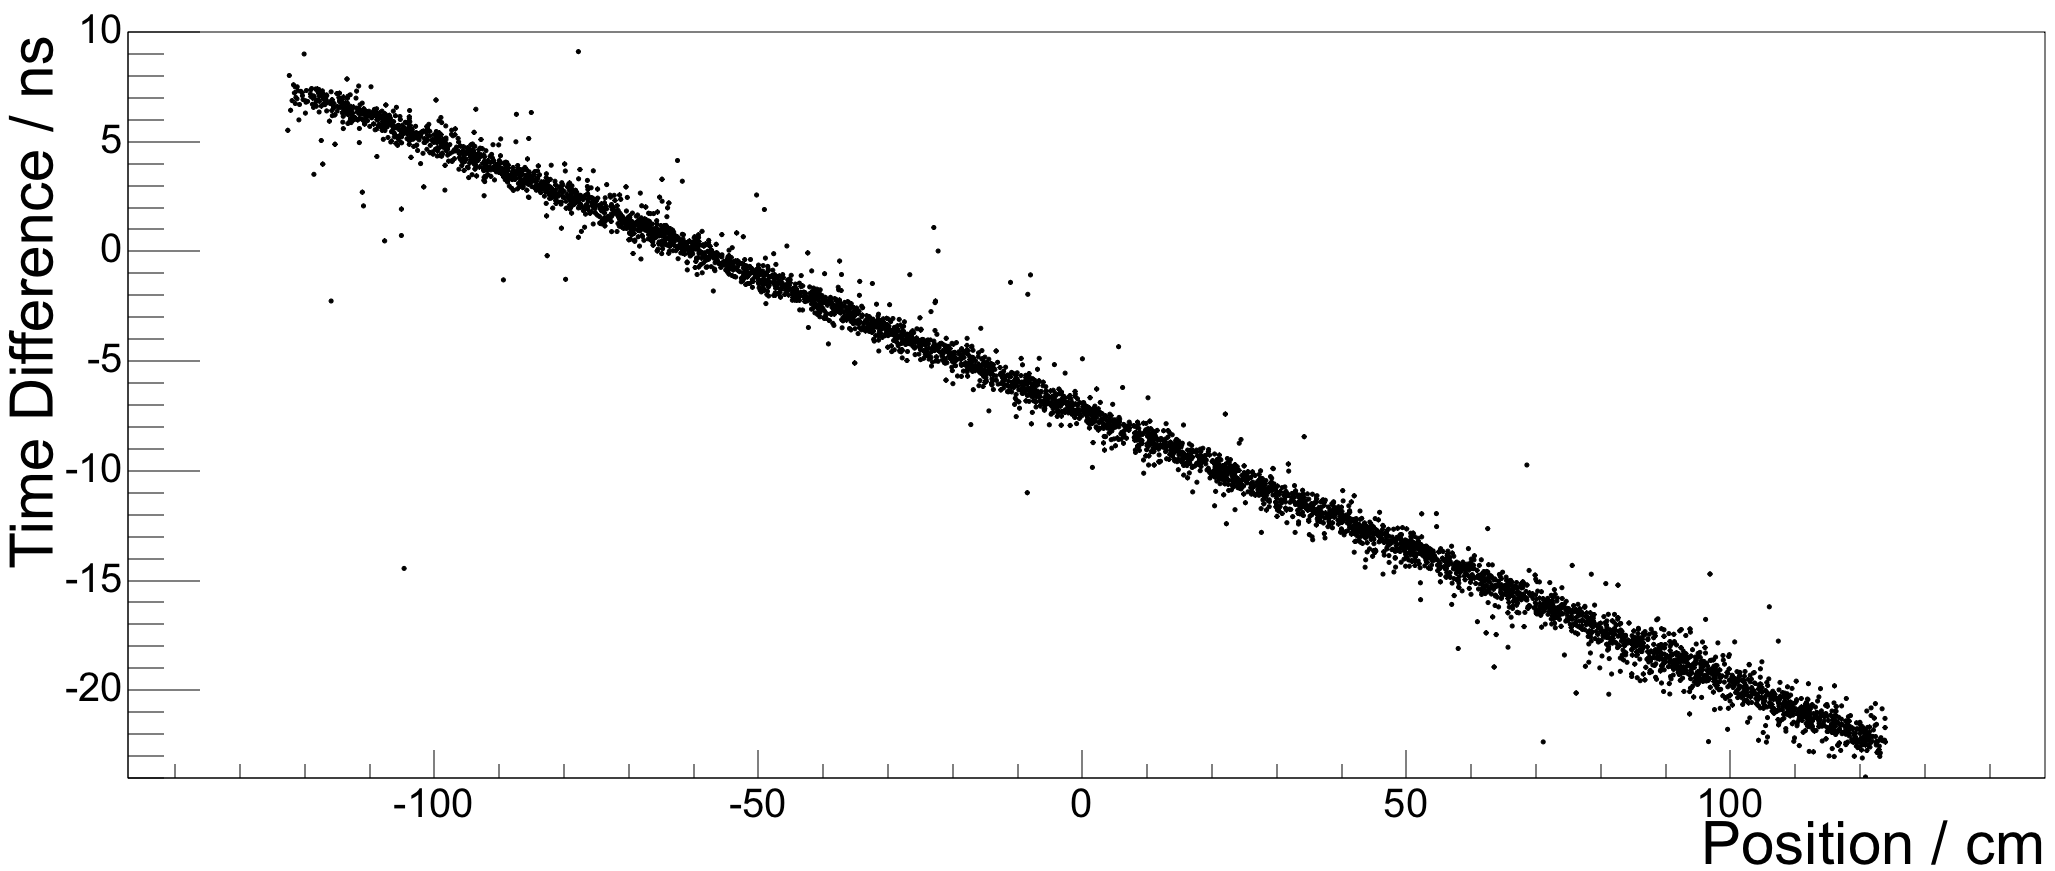
\includegraphics[ width = \textwidth]{R3BCon2024GSI/time_cal.png}
% 				\end{figure}
% 			}
% 		\end{column}
% 	\end{columns}
% \end{frame}

% \begin{frame}[t]{Position, time and energy calibration parameters}
% 	\vspace*{-1em}
% 	\begin{columns}
% 		\begin{column}{0.4 \textwidth}
% 			\begin{figure}[t]
% 				\centering
% 				\vspace*{-0.5em}
% 				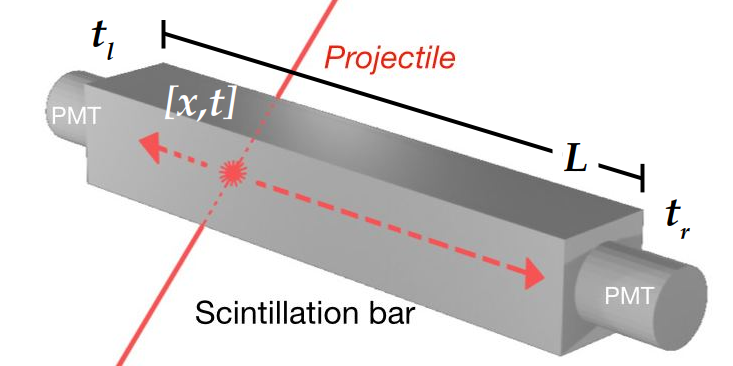
\includegraphics[width = \textwidth]{R3BCon2024GSI/Bar.png}
% 				\captionsetup{singlelinecheck=off,font=footnotesize}
% 				\vspace*{0.2em}
% 				\caption*{\textit{PMT saturation effect\footfullcite{Hamamatsu}:}}
% 				\vspace*{-1em}
% 				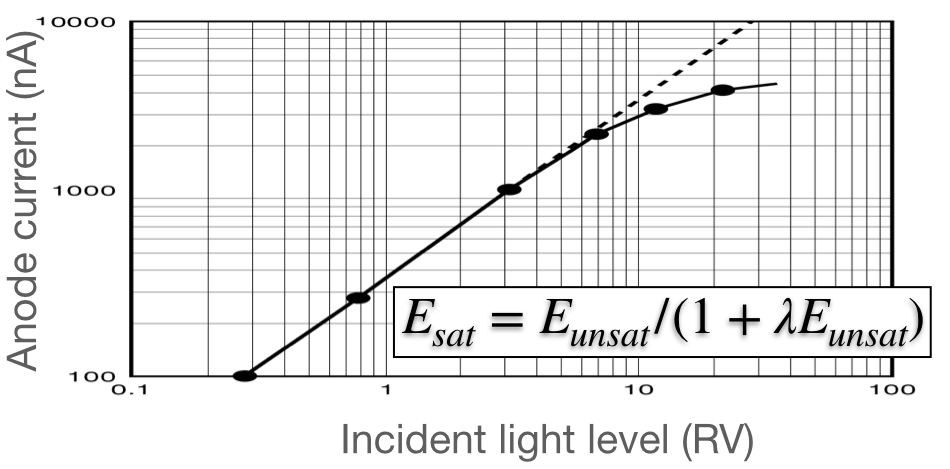
\includegraphics[width = \textwidth]{neuland/PMTSAT.png}
% 			\end{figure}
% 			\vspace{-1em}
% 		\end{column}
% 		\begin{column}{0.48 \textwidth}
% 			\vspace{-1em}
% 			\begin{block}{Position-Time calibration:}
% 				\setlength{\abovedisplayskip}{0pt}
% 				\setlength{\belowdisplayskip}{0pt}
% 				\setlength{\abovedisplayshortskip}{0pt}
% 				\setlength{\belowdisplayshortskip}{0pt}
% 				\begin{flalign*}
% 					\intertext{Interaction time:}
% 					t & = \frac{t_r + t_l}{2} - \frac{L}{2 \cdot \alert{C_e}} + \alert{t_\text{sync}} \\
% 					\intertext{Interaction position:}
% 					x & = \frac{\alert{C_e}}{2}\left( t_r - t_l  + \alert{t_\text{offset}} \right)
% 				\end{flalign*}
% 			\end{block}
% 			\vspace{-0.5em}
% 			\pause
% 			\begin{alertblock}{Energy calibration relations:}
% 				\setlength{\abovedisplayskip}{0pt}
% 				\setlength{\belowdisplayskip}{0pt}
% 				\setlength{\abovedisplayshortskip}{0pt}
% 				\setlength{\belowdisplayshortskip}{0pt}
% 				\begin{flalign*}
% 					\intertext{Light attenuation effect:}
% 					I_\text{PMT} & = E_\text{dep} \cdot \exp(-\alert{\alpha} \cdot l)                           \\
% 					\intertext{PMT saturation:}
% 					I_\text{sat} & = I_\text{PMT} \cdot / \left( 1 + \alert{\lambda} \cdot I_\text{PMT} \right) \\
% 					\intertext{PMT gain:}
% 					W            & = \alert{\mathcal{G}} \cdot I_\text{sat} + \alert{W_0}
% 				\end{flalign*}
% 			\end{alertblock}
% 		\end{column}
% 	\end{columns}
% \end{frame}

\end{document}
